
\section{Experimental setup}

The experimental setup used to measure the index of refraction for various gases is illustrated in Fig. \ref{fig:experimentalSetup}. The HeNe-laser beam is divided into two legs, reference leg $L_1$ and signal leg $L_2$ via a beam splitter (BS). The beam travelling down the signal leg is transmitted through a gas chamber made of acryllic glas, with inner length $d=100(1)$ mm. And then reflected via a mirror back the same way where it is reflected on the beam splitter where it coincides with the other part which has been reflected in $L_1$. The recombined laser beam shines through a small apperature in order to elliminate laser beams due to unwanted reflections. It then reaches a lens which diverges the laser beam in order to increase the resolution. A photodiode is mounted after the lens in order to pick up any changes of incident intensity of the combined laser beam. In order to eliminate ethalons inside the gas chamber, it was mounted at an angle relative the incident laser beam.

If the two legs are aligned propertly, an interferance pattern will emerge on the photodiode. If vaccum is created inside the gas chamber and then a steady flow of gas added, the optical path will increase. An interferance pattern (fringes) on the photodiode  will start to move continuously. By measuring the intensity changes 




\begin{figure}[H]
  \centering
  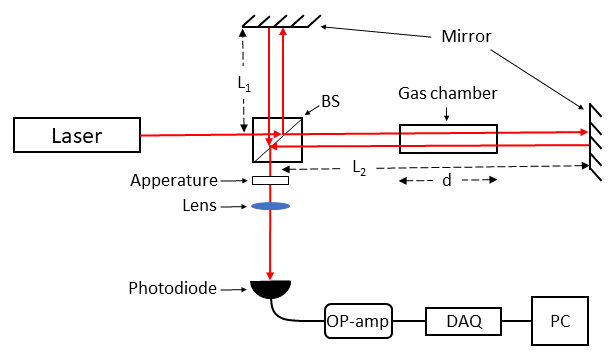
\includegraphics[width=0.8\textwidth]{Exp_setup.png}
  \caption{Experimental setup. }
  \label{fig:experimentalSetup}
\end{figure}
